%%%%%%%%%%%%%%%%%%%%%%
% Wenneker Resume/CV %
%%%%%%%%%%%%%%%%%%%%%%
\documentclass[a4paper,12pt]{memoir} % Font and paper size

\usepackage{multirow}
\input{structure.tex} % Include the file specifying document layout and packages

%----------------------------------------------------------------------------------------
%	NAME AND CONTACT INFORMATION 
%----------------------------------------------------------------------------------------

\userinformation{ % Set the content that goes into the sidebar of each page
\begin{flushright}
% Comment out this figure block if you don't want a photo
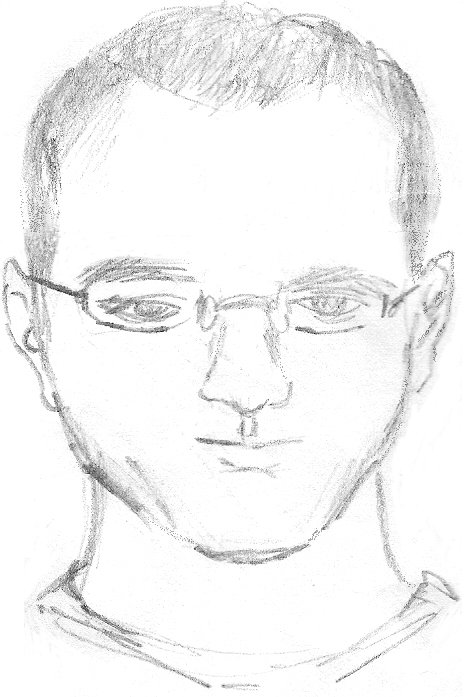
\includegraphics[width=\columnwidth]{lex.png}\\[\baselineskip] % Your photo
\large \textbf{Alex Towell} \\
\small \href{mailto:lex@metafunctor.com}{lex@metafunctor.com} \\
\vspace{0.5cm}
\href{https://metafunctor.com}{metafunctor.com} \\
\href{https://github.com/queelius}{github.com/queelius} \\
\vspace{0.5cm}
(618) 977-1746 \\ % Your phone number
\vfill % Whitespace under this block to push it up under the photo
\end{flushright}
}

%----------------------------------------------------------------------------------------

\begin{document}

\userinformation % Print your information in the left column

\framebreak % End of the first column

%----------------------------------------------------------------------------------------
%	HEADING
%----------------------------------------------------------------------------------------

\cvheading{Alex Towell} % Large heading - your name

\cvsubheading{PhD Student | AI Researcher | Mathematician}

%-------------------------------------------------------------------------
%----------------------------------------------------------------------------------------
%	ABOUT ME
%----------------------------------------------------------------------------------------

\aboutme{About Me}{PhD student in Computer Science at Southern Illinois University, specializing in AI safety, alignment, and cybersecurity. Leading ransomware prevention research achieving $10^{-8}$ false-negative rates. Architecting production systems for Illinois DOT while maintaining 100+ open-source projects in AI, cryptography, and mathematics. Seeking to contribute to cutting-edge AI research with real-world impact.}

%----------------------------------------------------------------------------------------
%	EDUCATION
%----------------------------------------------------------------------------------------

\CVSection{Education}

\CVItem{2024 - Present, Southern Illinois University}{PhD in Computer Science}
{
    \begin{itemize}
        \item Research Focus: Cybersecurity, AI Safety, Alignment, Machine Learning
        \item Advisor: Dr. Hiroshi Fujinoki
        \item Expected Graduation: 2028
    \end{itemize}
}

\Sep

%------------------------------------------------

\CVItem{2021 - 2023, Southern Illinois University-Edwardsville}{MS in Mathematics}
{
    \begin{itemize}
        \item GPA: 3.9/4.0
        \item Concentration: Statistics and Operations Research
        \item Awarded R.N. Pendergrass Graduate Scholarship
    \end{itemize}
}

\Sep

%------------------------------------------------

\CVItem{2012 - 2015, Southern Illinois University-Edwardsville}{MS in Computer Science}
{
    \begin{itemize}
        \item GPA: 4.0/4.0
        \item Concentration: Artificial Intelligence
        \item Awarded Outstanding Graduate Student (School of Engineering)
    \end{itemize}
}

\Sep

%------------------------------------------------

\CVItem{2006 - 2010, Southern Illinois University-Edwardsville}{BS in Computer Science}
{
    \begin{itemize}
        \item GPA: 3.6/4.0
        \item Awarded Outstanding Junior (Dept. of Computer Science)
    \end{itemize}
}

%------------------------------------------------

\Sep

%----------------------------------------------------------------------------------------
% TECHNICAL SKILLS
%----------------------------------------------------------------------------------------

\CVSection{Technical Skills}

\CVItem{Languages}{Python, R, C/C++, Java, Scala, JavaScript, TypeScript, Bash}\\
\CVItem{AI/ML}{PyTorch, HuggingFace, CUDA, LangChain, Fine-Tuning, Transformers}\\
\CVItem{Systems}{Linux, Docker, Git, PostgreSQL, Elasticsearch, Redis, REST APIs}\\
\CVItem{Cryptography}{Encrypted Search, Secure Indexes, Oblivious Computing, Bloom Filters}\\
\CVItem{Frameworks}{React, Node.js, FastAPI, Flask, Jupyter, LaTeX}

\clearpage % Start a new page

\userinformation % Print your information in the left column

\framebreak % End of the first column

%----------------------------------------------------------------------------------------
%	PUBLICATIONS
%----------------------------------------------------------------------------------------

\CVSection{Publications}

\begin{itemize}
    \item H. Fujinoki, \textbf{A. Towell}, V.A. Thota, ``Preventing Ransomware Damages using In-Operation Off-Site Backup to Achieve a $10^{-8}$ False-Negative Miss-Detection Rate,'' \textit{International Conference on Computing and Intelligence (ICCI)}, 2025
    \item \textbf{A. Towell}, ``Reliability Estimation in Series Systems: Maximum Likelihood Techniques for Right-Censored and Masked Failure Data,'' Master's Project, Department of Mathematics and Statistics, Southern Illinois University Edwardsville, 2023
    \item \textbf{A. Towell}, H. Fujinoki, ``Estimating How Confidential Encrypted Searches Are Using Moving Average Bootstrap Method,'' \textit{IEEE International Conference on Cloud Computing Technology and Science (CloudCom)}, 2016
    \item \textbf{A. Towell}, ``Encrypted Search: Enabling Standard Information Retrieval Techniques Using New Secure Index Types,'' Master's Thesis, ProQuest Dissertations \& Theses, 2015
\end{itemize}

\Sep

%----------------------------------------------------------------------------------------
% SELECTED RESEARCH AND PROJECTS
%----------------------------------------------------------------------------------------

\CVSection{Selected Research \& Projects}

\CVItem{AlgoTree}{Developed a Python package offering utilities for tree-like data structures, including FlatForest and TreeNode representations. Features a command-line tool \texttt{jt} for creating, manipulating, querying, and visualizing trees, akin to \texttt{jq} but tailored for hierarchical data.}\\
\CVItem{Elasticsearch-LM}{Fine-tuning smaller Large Language Models (LLMs) for translating natural language queries into structured Elasticsearch Query DSL. Emphasizes synthetic data generation to enhance model training, aiming to democratize sophisticated API interactions.}\\
\CVItem{Reverse-Process Synthetic Data Generation}{Developed novel algorithms generating synthetic data via reverse-process methods to facilitate LLM-based mathematical reasoning and theorem proving. Focus on creating high-quality training data for complex reasoning tasks.}\\
\CVItem{Oblivious Computation}{Researching cryptographic methods enabling secure computation trade-offs between space and security without full homomorphism. Applications in privacy-preserving cloud computing.}\\
\CVItem{IDOT D8 Infrastructure System}{Architected and implemented comprehensive full-stack application for traffic monitoring and infrastructure management. Large-scale production system handling real-time data processing for Illinois transportation.}

\clearpage % Start a new page

\userinformation % Print your information in the left column

\framebreak % End of the first column

%----------------------------------------------------------------------------------------
% ACADEMIC EXPERIENCE
%----------------------------------------------------------------------------------------

\CVSection{Academic Experience}

\CVItem{2024--Present, Research Assistant, SIU}{
    \begin{itemize}
        \item Research in cybersecurity under Dr. Hiroshi Fujinoki, focusing on ransomware detection and prevention using probabilistic data structures and backup strategies
        \item Lead developer for Illinois Department of Transportation District 8 (IDOT D8) full-stack application
        \item Developed large-scale codebase for traffic data processing and infrastructure management systems
        \item Co-authored paper on achieving $10^{-8}$ false-negative miss-detection rates in ransomware prevention (ICCI 2025)
    \end{itemize}
}

\Sep

\CVItem{2021--2022, Teaching Assistant, SIUE}{
    \begin{itemize}
        \item Taught lab courses in mathematics and statistics
    \end{itemize}
}

\Sep

\CVItem{2012--2015, Research/Graduate/Teaching Assistant, SIUE}{
    \begin{itemize}
        \item Supported research in AI and machine learning while pursuing MS in Computer Science
        \item Taught undergraduate computer science lab sessions
        \item Developed encrypted search algorithms for confidential data retrieval systems
    \end{itemize}
}

\end{document}